\section{Ergebnisse}
In diesem Kapitel werden die Ergebnisse des Projektes vorgestellt. Dabei werden sowohl der Verlauf der Implementierungsphase als auch die finalen Ergebnisse behandelt. Zunächst wurde ein Prototyp entwickelt, der die wesentlichen Funktionalitäten der Künstlichen Intelligenz und der Spielumgebung beinhaltet, um sicherzustellen, dass das Vorhaben im Rahmen der Vorgaben umsetzbar ist und um Einblicke in möglichen Problemstellungen des Vorhabens zu gewinnen. Danach wurde der Prototyp schrittweise erweitert, bis schließlich das komplette Spiel mit allen Funktionalitäten umgesetzt worden ist und die Künstliche Intelligenz mit diesem trainiert werden konnte.
\subsection{Trainingshistorie}
\subsubsection{Prototyp}
Bei dieser Version handelt es sich um den ersten lauffähigen Prototypen. Es wurde nur eines der farbigen Felder (gelb) in der Spielumgebung implementiert. Das Modell kann mithilfe dieser Spielumgebung bereits trainiert werden und erzielt zum Teil gute Punktezahlen.\\

Abbildung 11 zeigt das die Punktestände des ersten erfolgreiche Trainings des Modells für 27000 Episoden:
\nopagebreak
\begin{figure}[H]
	\centering
	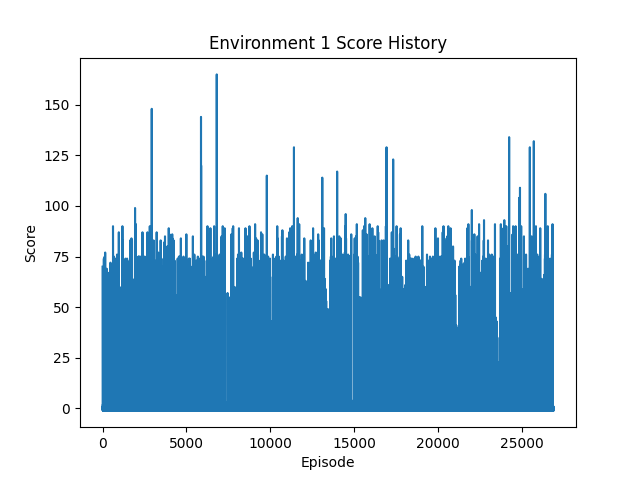
\includegraphics[width=0.8\textwidth]{Bilder/firstpropertraining} 
	\caption[Punktezahlen des ersten trainierten Modells für 27000 Episoden]{Punktezahlen des ersten trainierten Modells für 27000 Episoden\\ Quelle: Eigene Darstellung}
\end{figure}

Das Modell erreicht innerhalb einer Episode (eines Spiels) oft eine Punktzahl von 70. Teilweise erreicht es sogar mehr als 150 Punkte. Fragwürdig ist dabei, dass die maximale Punktzahl zu diesem Zeitpunkt bei 86 liegen sollte, das Modell jedoch gelegentlich höhere Punktzahlen erzielt. Dies war darauf zurückzuführen, dass die Spielumgebung erzielte Punkte teilweise mehrfach anrechnete und somit mehr Punkte zu erspielen waren, als vorgesehen.\\

Abbildung 12 zeigt die Punktestände des ersten erfolgreiche Trainings des Modells für 45 Episoden:
\nopagebreak
\begin{figure}[H]
	\centering
	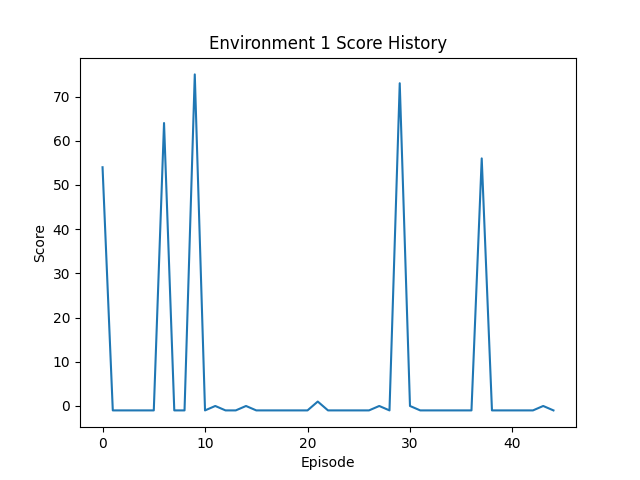
\includegraphics[width=0.8\textwidth]{Bilder/firstpropertraining100steps} 
	\caption[Punktezahlen des ersten trainierten Modells für 45 Episoden]{Punktezahlen des ersten trainierten Modells für 45 Episoden\\ Quelle: Eigene Darstellung}
\end{figure}

Abbildung 12 zeigt, dass das Modell in dieser Version zwar teilweise eine gute Menge an Punkten erzielt, im Großteil der Spiele allerdings nur null oder einen bis zwei Punkte erzielt. Dies ist darauf zurückzuführen, dass die Spielumgebung bei dieser Version das Spiel unverzüglich beendet, wenn eine ungültige Aktion gewählt wird. Daraus ist zu schließen, dass das Modell überwiegend ungültige Aktionen wählt, da bei nur 100 ausgeführten Schritten bereits 45 Spiele abgeschlossen wurden. Vorgesehen sind zu diesem Zeitpunkt pro Spiel zehn Spielschritte. Somit wurden mehr als vier mal so viele Spiele abgeschlossen als unter optimalen Bedingungen vorgesehen.
\subsubsection{Training mit und ohne Aktionsmaske}
Abbildung 13 zeigt die erzielten Punkte des Modells ohne Aktionsmaske für 20 Episoden:
\nopagebreak
\begin{figure}[H]
	\centering
	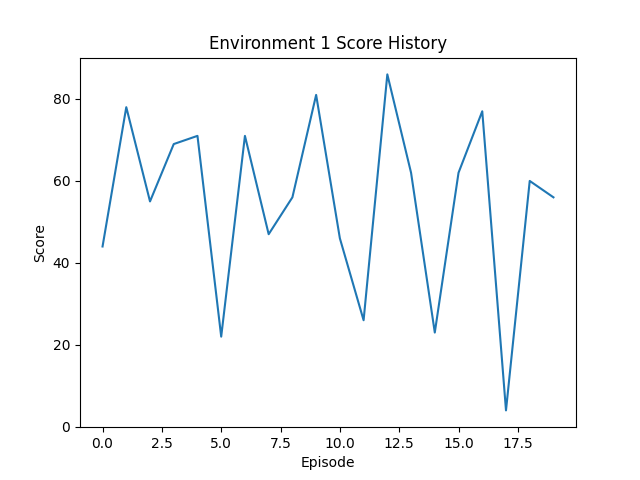
\includegraphics[width=0.8\textwidth]{Bilder/trainingwithoutcancalation} 
	\caption[Punktezahlen des Modells ohne Aktionsmaske für 20 Episoden]{Punktezahlen des Modells ohne Aktionsmaske für 20 Episoden\\ Quelle: Eigene Darstellung}
\end{figure}

Das anfängliche Verfahren bei dem das Spiel beendet wurde, sobald eine ungültige Aktion gewählt wurde, stellte sich als nicht geeignet heraus, da das Modell immer wieder ungültige Aktionen wählte, was zum Abbruch vieler Spielrunden führte. Daher wurde ein Trainingsverfahren mit negativer Belohnung bei ungültigen und positiver bei gültigen Aktionen gewählt. Diese Belohnungen sind in Abbildung 13 nicht zu sehen, da sie herausgefiltert worden sind. Abbildung 13 zeigt nur die aufsummierten Belohnungen, die 10 oder mehr Punkte betragen. Diese Belohnungen entsprechen den Belohnungen des gelben Feldes, welche mindestens 10 bis maximal 20 Punkte betragen. Insgesamt zeigt sich eine verhältnismäßig gute Performanz bei der das Modell im Durchschnitt um die 50 Punkte erzielt. Bedenkt man, dass das Maximum bei 86 Punkten liegt und ungültige Aktionen getätigt werden können ist dieses Ergebnis gut. Das Modell erzielt im Durchschnitt ungefähr 60 Prozent der maximal erreichbaren Punktezahl.\\

Abbildung 14 zeigt die erzielten Punkte des Modells mit Aktionsmaske für 20 Episoden:
\nopagebreak
\begin{figure}[H]
	\centering
	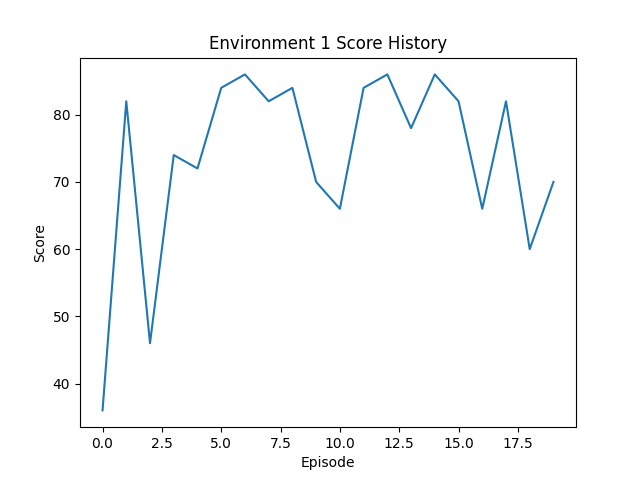
\includegraphics[width=0.8\textwidth]{Bilder/trainingwithactionmask} 
	\caption[Punktezahlen des Modells mit Aktionsmaske für 20 Episoden]{Punktezahlen des Modells mit Aktionsmaske für 20 Episoden\\ Quelle: Eigene Darstellung}
\end{figure}

Die Performanz hat im Gegensatz zur Variante ohne Aktionsmaske zugenommen. Das Modell erzielt im Durchschnitt ungefähr 65 Punkte was einem Zuwachs von ungefähr einem Drittel entspricht. Die erzielten Punkte steigen somit von ungefähr 60 Prozent des Maximums auf 75 Prozent. Die Performanz des Vorgängermodells den Umständen entsprechend gut, allerdings erzielt die Variante mit Aktionsmaske ohne größere Umstände ein wesentlich besseres Ergebnis. Deshalb wurde das Projekt ab diesem Zeitpunkt mit Aktionsmaske fortgesetzt.
\subsubsection{Training mit zwei und vier Würfeln}
Abbildung 15 zeigt die ungültigen Züge einer Spielsimulation mit zwei Würfeln für 20 Episoden:
\nopagebreak
\begin{figure}[H]
	\centering
	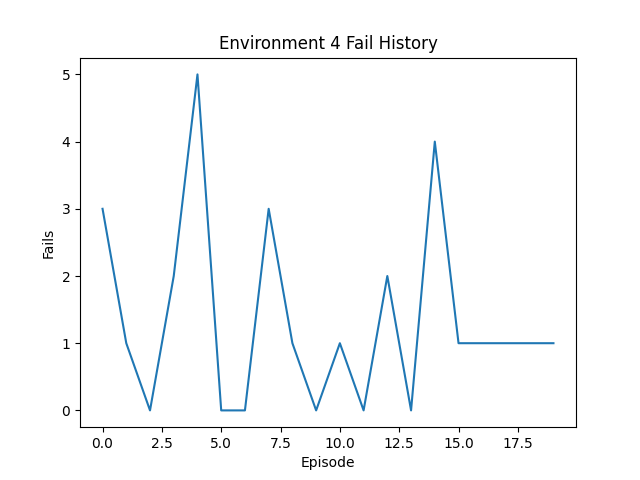
\includegraphics[width=0.8\textwidth]{Bilder/failswithtwodice} 
	\caption[Ungültige Züge des Modells unter Verwendung von zwei Würfeln für 20 Episoden]{Ungültige Züge des Modells unter Verwendung von zwei Würfeln für 20 Episoden\\ Quelle: Eigene Darstellung}
\end{figure}

Das Modell wählt von null bis fünf ungültige Aktionen pro Spiel. Es ergibt sich ein Durchschnitt von ungefähr 1-2 ungültigen Zügen pro Spiel. Dies sollte nicht auftreten, wenn dem Modell keine ungültigen Aktionen zur Verfügung stehen. Die Aktionsmaske sorgt dafür, dass unter normalen Umständen nur gültige Aktionen gewählt werden können. Das Problem entsteht, wenn dem Modell keine gültigen Aktionen zur Auswahl stehen. In diesem Fall wählt das Modell eine zufällige Aktion und berücksichtigt die Aktionsmaske nicht. Da in dieser Version nur zwei Würfel zur Verfügung stehen kommt es oft zu dem Fall, dass keiner der Würfel zu einem der Felder passt und somit kann keines der Kästchen ausgefüllt werden. Dadurch steht keine gültige Aktion zur Verfügung und es wird eine ungültige Aktion gewählt.\\

Abbildung 16 zeigt die ungültigen Züge einer Spielsimulation mit vier Würfeln für 20 Episoden:
\nopagebreak
\begin{figure}[H]
	\centering
	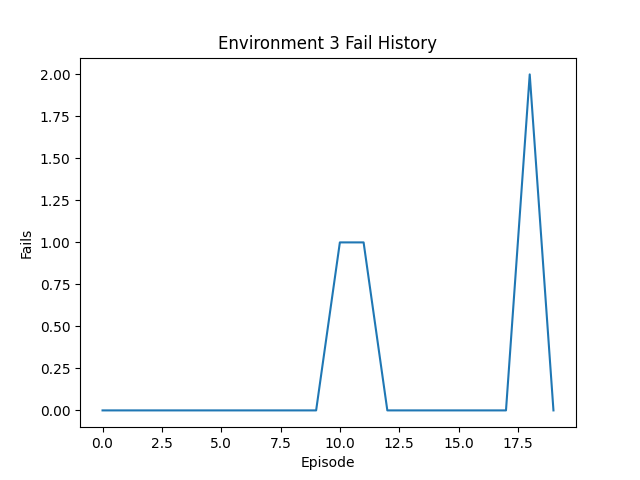
\includegraphics[width=0.8\textwidth]{Bilder/failswithfourdice} 
	\caption[Ungültige Züge des Modells unter Verwendung von vier Würfeln für 20 Episoden]{Ungültige Züge des Modells unter Verwendung von vier Würfeln für 20 Episoden\\ Quelle: Eigene Darstellung}
\end{figure}

Die Anzahl an ungültigen Zügen hat im Gegensatz zur Variante mit zwei Würfeln drastisch abgenommen. Zwar kommt es vereinzelt immer noch zu Fällen bei denen das Modell ungültige Aktionen wählen muss, allerdings ist die Wahrscheinlichkeit dafür bei vier Würfeln deutlich geringer.
\subsubsection{Optimiertes Training}
Abbildung 17 zeigt die erzielten Punkte des Modells nachdem eine Vielzahl an Optimierungen vorgenommen wurden:
\nopagebreak
\begin{figure}[H]
	\centering
	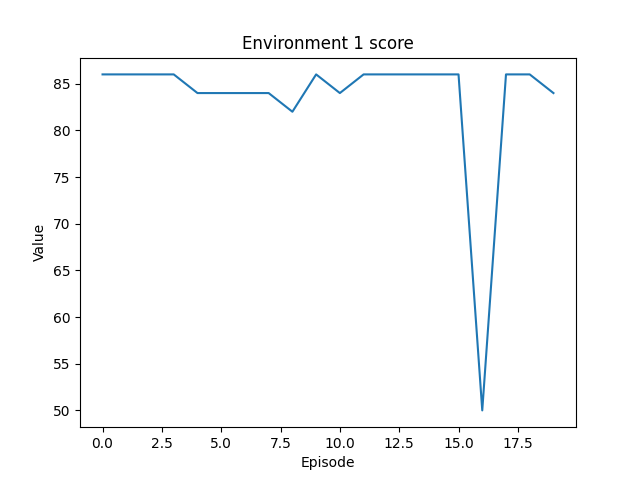
\includegraphics[width=0.8\textwidth]{Bilder/optimizetraining} 
	\caption[Punktezahlen des Modells nach optimiertem Training für 20 Episoden]{Punktezahlen des Modells nach optimiertem Training für 20 Episoden\\ Quelle: Eigene Darstellung}
\end{figure}

Abbildung 17 zeigt, dass das Modell im Durchschnitt etwas mehr als 80 Punkte erzielt hat. Dies ist ein sehr guter Wert, da die maximale Punktezahl bei 86 liegt. Die maximale Punktezahl von 86 Punkten wurde innerhalb der zwanzig Episoden zehn mal erreicht.
\subsection{Erstes Training mit allen Feldern und Boni}
Abbildung 18 zeigt die Ergebnisse des ersten Trainings mit einer Spielumgebung bei der alle farbigen Felder und Boni implementiert worden sind:
\nopagebreak
\begin{figure}[H]
	\centering
	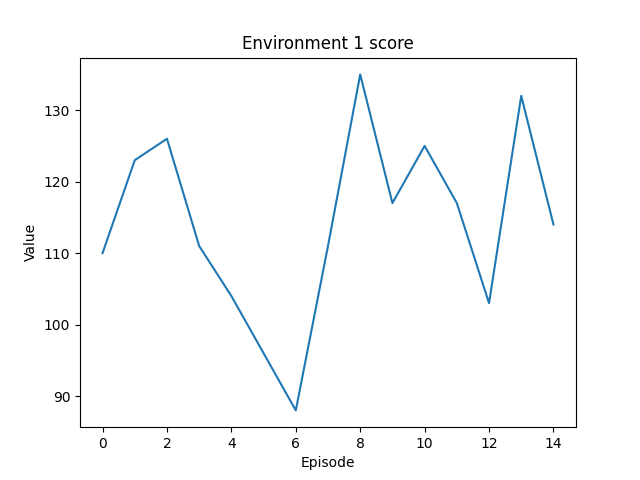
\includegraphics[width=0.8\textwidth]{Bilder/firsttrainingwithallfields} 
	\caption[Punktezahlen des erstes trainierten Modells mit allen Feldern]{Punktezahlen des erstes trainierten Modells mit allen Feldern\\ Quelle: Eigene Darstellung}
\end{figure}

Abbildung 18 zeigt, dass das Modell bereits Werte im Bereich von 89 bis 134 Punkten erzielt, allerdings lässt sich an dieser Stelle noch viel optimieren. Im Schnitt erzielt es etwas mehr als 110 Punkte. So viele Punkte erzielt im Allgemeinen auch ein menschlicher Neueinsteiger, der das Spiel kaum kennt. Bei dieser Version des Spiels gibt es noch viele Bugs, die dazu führen, dass weniger Punkte erspielt werden, als es unter ordentlichen Bedingungen möglich wäre.
\subsection{Finale Ergebnisse}
\subsubsection{Performanz}
Abbildung 19 zeigt die erzielten Punktezahlen des Modells nach dem finalen Training für 1000 Episoden:
\nopagebreak
\begin{figure}[H]
	\centering
	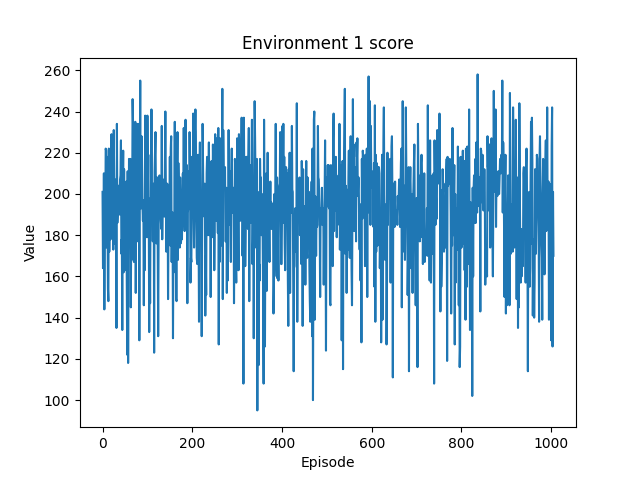
\includegraphics[width=0.8\textwidth]{Bilder/maskableppo_ganzschoenclever_193avg_v3.1} 
	\caption[Punktezahlen des finalen Modells für 1000 Episoden]{Punktezahlen des finalen Modells für 1000 Episoden\\ Quelle: Eigene Darstellung}
\end{figure}

Abbildung 19 zeigt, dass das Modell über einen Zeitraum von mehr als 1000 Episoden eine durchschnittliche Punktezahl von ungefähr 205 Punkten erzielt. Das ist beachtlich, da menschliche Spieler in einem Versuch im Durchschnitt lediglich 175,75 Punkte erzielen konnten.\\

Abbildung 20 zeigt die ungültigen Züge des Modells nach dem finalen Training für 1000 Episoden:
\nopagebreak
\begin{figure}[H]
	\centering
	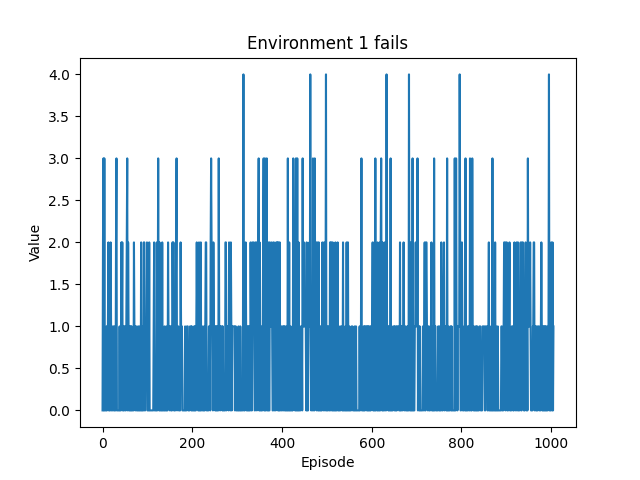
\includegraphics[width=0.8\textwidth]{Bilder/maskableppo_ganzschoenclever_193avg_v3.1f}
	\caption[Ungültige Züge des finalen Modells für 1000 Episoden]{Ungültige Züge des finalen Modells für 1000 Episoden\\ Quelle: Eigene Darstellung}
\end{figure}

Abbildung 20 zeigt, dass das Modell in den meisten Fällen maximal einen ungültigen Zug tätigt. Teilweise werden noch zwei ungültige Züge pro Episode ausgeführt und noch seltener drei oder vier. Angesichts dessen, dass das Modell pro Spielrunde ungefähr 40 Züge machte und häufig Würfel bei einer Wahl ungültig gemacht werden können, ist das ein beachtliches Ergebnis. Das Modell lernte es Verhaltensweisen zu vermeiden, die dazu führen, dass keine gültigen Aktionen zur Auswahl stehen.\\

Die Abbildungen 21 und 22 zeigen die erzielten Punktestände und ungültigen Züge des finalen Modells für 100 Episoden. Die Abbildungen sind anschaulicher als die Abbildungen für 1000 Episoden:
\nopagebreak
\begin{figure}[H]
	\centering
	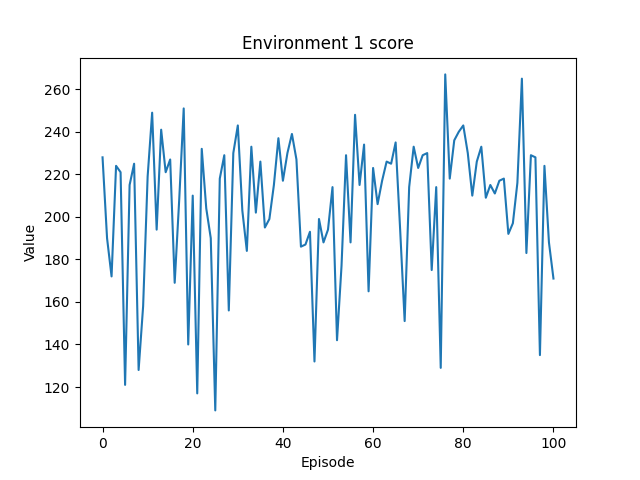
\includegraphics[width=0.8\textwidth]{Bilder/final4000steps} 
	\caption[Punktezahlen des finalen Modells für 100 Episoden]{Punktezahlen des finalen Modells für 100 Episoden\\ Quelle: Eigene Darstellung}
\end{figure}
\begin{figure}[H]
	\centering
	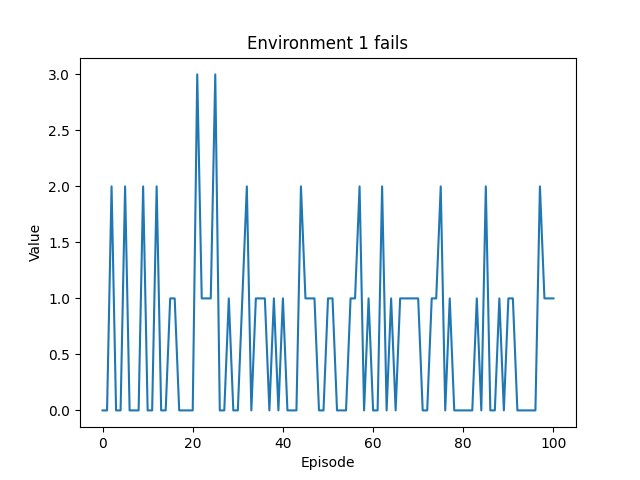
\includegraphics[width=0.8\textwidth]{Bilder/final4000stepsf} 
	\caption[Ungültige Züge des finalen Modells für 100 Episoden]{Ungültige Züge des finalen Modells für 100 Episoden\\ Quelle: Eigene Darstellung}
\end{figure}
\subsubsection{Finale Hyperparameter und Performanzwerte}
Die Hyperparameter für das finale Training sind:

\begin{itemize} 
\item Ein neuronale Netz mit sieben Schichten von jeweils 1024 Neuronen. 

\item Ein Gamma von 1. 

\item Ein Entropie-Koeffizient von 0.1. 

\item Eine Lernrate von 0.0006. 

\item Eine Clip Range von 0.2. 

\item Eine Umgebungsanzahl von 32. 

\item Datenpakete mit 2048 Aktions-Zustands-Paaren, welche jeweils 5 Mal verwendet werden und dabei in Batches von 128 Aktions-Zustands-Paaren aufgeteilt werden. 

\item Ein Entropie-Koeffizient von 0 für das Verfestigen des gelernten Verhaltens. 
\end{itemize} 

Das Modell wurde in diesem Prozess zunächst für 2.220.000 Zeitschritte trainiert. Daraufhin wurde es mit dem Entropie-Koeffizient von 0 für weitere 1.110.000 Zeitschritte trainiert, um das gelernte Verhalten weiter zu verfestigen. Dieser Prozess wurde dann zwei weitere Male mit doppelt so vielen Zeitschritten wiederholt. Zunächst betrug die durchschnittliche Punktezahl des Modells 192,26, danach 201,04 und schließlich 204,98. Die Standardabweichung im letzten Test lag bei 31,22 und der Median bei 211. Vergleichsweise erzielten menschliche Spieler in einem Test durchschnittlich 175,75 Punkte mit einer Standardabweichung von 26,75. Ein fortgeschrittener menschlicher Spieler erzielte im Durchschnitt 215,75 Punkte. Dabei ist zu beachten, dass die Künstliche Intelligenz im Nachteil ist, da ihr unter anderem am Ende des Spiels eine Wahl vom Silbertablett und somit ein ausgefülltes Kästchen fehlt [s. Abschnitt 4.1].

Für die durchschnittlichen Punktezahlen der Künstlichen Intelligenz, wurden die erreichten Punkte einer abgeschlossenen Spielumgebung abgespeichert, anschließend aufaddiert und durch ihre Anzahl geteilt. Einmalig erzielte die Künstliche Intelligenz 282 Punkte, was laut der offiziellen Punkteskala von Schmidt Spiele dem höchsten Level an Performanz entspricht \cite{schmidtspiele_ganzschonclever}.
\subsubsection{ChatGPT 4}
ChatGPT 4 [s. Unterabschnitt 2.2.4] wurde verwendet, um den Prototypen des Projektes bis zu seinem ersten erfolgreichen Einsatz zu implementieren. Dabei hat es sich als besonders nützlich erwiesen, um einen lauffähigen Code mit den gewünschten, relativ simplen Methoden zu implementieren. Dies ist besonders bei der Erstellung eines ersten Prototypen, oder um die Machbarkeit eines Projektes zu überprüfen, vorteilhaft. Im späteren Verlauf wurden von ChatGPT 4 generierte Inhalte nicht mehr direkt übernommen. ChatGPT 4 wurde in weiteren Verlauf lediglich benutzt, um Auskunft über geeignete oder bereits verwendete Technologien zu geben, Ideen zu sammeln oder Syntax zu erfragen. Auch für diese Aufgaben stellte sich ChatGPT 4 als sehr nützlich heraus. Solange die Fragen nicht zu spezifisch oder komplex waren lieferte ChatGPT 4 häufig gute und hilfreiche Antworten. Ist die Problemstellung zu komplex oder zu spezifisch, scheint ChatGPT 4 Schwierigkeiten zu haben eine vollständige oder geeignete Antwort zu liefern. Außerdem ist die Datenbank des ChatGPT 4 Modells auf den September 2021 datiert, was den Nutzen für neuere Sachverhalte erschwert.